\PassOptionsToPackage{unicode=true}{hyperref} % options for packages loaded elsewhere
\PassOptionsToPackage{hyphens}{url}
%
\documentclass[10pt,xcolor=table,color={dvipsnames,usenames},ignorenonframetext,usepdftitle=false,french]{beamer}
\setbeamertemplate{caption}[numbered]
\setbeamertemplate{caption label separator}{: }
\setbeamercolor{caption name}{fg=normal text.fg}
\beamertemplatenavigationsymbolsempty
\usepackage{caption}
\captionsetup{skip=0pt,belowskip=0pt}
%\setlength\abovecaptionskip{-15pt}
\usepackage{lmodern}
\usepackage{amssymb,amsmath,mathtools,multirow}
\usepackage{float,hhline}
\usepackage{tikz}
\usepackage{mathtools}
\usepackage{ifxetex,ifluatex}
\usepackage{fixltx2e} % provides \textsubscript
\ifnum 0\ifxetex 1\fi\ifluatex 1\fi=0 % if pdftex
  \usepackage[T1]{fontenc}
  \usepackage[utf8]{inputenc}
  \usepackage{textcomp} % provides euro and other symbols
\else % if luatex or xelatex
  \usepackage{unicode-math}
  \defaultfontfeatures{Ligatures=TeX,Scale=MatchLowercase}
\fi
\usetheme[coding=utf8,language=english,
,titlepagelogo=img/logobeamer.png
]{TorinoTh}
% use upquote if available, for straight quotes in verbatim environments
\IfFileExists{upquote.sty}{\usepackage{upquote}}{}
% use microtype if available
\IfFileExists{microtype.sty}{%
\usepackage[]{microtype}
\UseMicrotypeSet[protrusion]{basicmath} % disable protrusion for tt fonts
}{}
\IfFileExists{parskip.sty}{%
\usepackage{parskip}
}{% else
\setlength{\parindent}{0pt}
\setlength{\parskip}{6pt plus 2pt minus 1pt}
}
\usepackage{hyperref}
\hypersetup{
            pdfauthor={Alain Quartier-la-Tente},
            pdfborder={0 0 0},
            breaklinks=true}
\urlstyle{same}  % don't use monospace font for urls
\newif\ifbibliography
\newlength{\cslhangindent}
\setlength{\cslhangindent}{1.5em}
\newlength{\csllabelwidth}
\setlength{\csllabelwidth}{3em}
\newenvironment{CSLReferences}[2] % #1 hanging-ident, #2 entry spacing
 {% don't indent paragraphs
  \setlength{\parindent}{0pt}
  % turn on hanging indent if param 1 is 1
  \ifodd #1 \everypar{\setlength{\hangindent}{\cslhangindent}}\ignorespaces\fi
  % set entry spacing
  \ifnum #2 > 0
  \setlength{\parskip}{#2\baselineskip}
  \fi
 }%
 {}
\usepackage{color}
\usepackage{fancyvrb}
\newcommand{\VerbBar}{|}
\newcommand{\VERB}{\Verb[commandchars=\\\{\}]}
\DefineVerbatimEnvironment{Highlighting}{Verbatim}{commandchars=\\\{\}}
% Add ',fontsize=\small' for more characters per line
\usepackage{framed}
\definecolor{shadecolor}{RGB}{248,248,248}
\newenvironment{Shaded}{\begin{snugshade}}{\end{snugshade}}
\newcommand{\AlertTok}[1]{\textcolor[rgb]{0.94,0.16,0.16}{#1}}
\newcommand{\AnnotationTok}[1]{\textcolor[rgb]{0.56,0.35,0.01}{\textbf{\textit{#1}}}}
\newcommand{\AttributeTok}[1]{\textcolor[rgb]{0.77,0.63,0.00}{#1}}
\newcommand{\BaseNTok}[1]{\textcolor[rgb]{0.00,0.00,0.81}{#1}}
\newcommand{\BuiltInTok}[1]{#1}
\newcommand{\CharTok}[1]{\textcolor[rgb]{0.31,0.60,0.02}{#1}}
\newcommand{\CommentTok}[1]{\textcolor[rgb]{0.56,0.35,0.01}{\textit{#1}}}
\newcommand{\CommentVarTok}[1]{\textcolor[rgb]{0.56,0.35,0.01}{\textbf{\textit{#1}}}}
\newcommand{\ConstantTok}[1]{\textcolor[rgb]{0.00,0.00,0.00}{#1}}
\newcommand{\ControlFlowTok}[1]{\textcolor[rgb]{0.13,0.29,0.53}{\textbf{#1}}}
\newcommand{\DataTypeTok}[1]{\textcolor[rgb]{0.13,0.29,0.53}{#1}}
\newcommand{\DecValTok}[1]{\textcolor[rgb]{0.00,0.00,0.81}{#1}}
\newcommand{\DocumentationTok}[1]{\textcolor[rgb]{0.56,0.35,0.01}{\textbf{\textit{#1}}}}
\newcommand{\ErrorTok}[1]{\textcolor[rgb]{0.64,0.00,0.00}{\textbf{#1}}}
\newcommand{\ExtensionTok}[1]{#1}
\newcommand{\FloatTok}[1]{\textcolor[rgb]{0.00,0.00,0.81}{#1}}
\newcommand{\FunctionTok}[1]{\textcolor[rgb]{0.00,0.00,0.00}{#1}}
\newcommand{\ImportTok}[1]{#1}
\newcommand{\InformationTok}[1]{\textcolor[rgb]{0.56,0.35,0.01}{\textbf{\textit{#1}}}}
\newcommand{\KeywordTok}[1]{\textcolor[rgb]{0.13,0.29,0.53}{\textbf{#1}}}
\newcommand{\NormalTok}[1]{#1}
\newcommand{\OperatorTok}[1]{\textcolor[rgb]{0.81,0.36,0.00}{\textbf{#1}}}
\newcommand{\OtherTok}[1]{\textcolor[rgb]{0.56,0.35,0.01}{#1}}
\newcommand{\PreprocessorTok}[1]{\textcolor[rgb]{0.56,0.35,0.01}{\textit{#1}}}
\newcommand{\RegionMarkerTok}[1]{#1}
\newcommand{\SpecialCharTok}[1]{\textcolor[rgb]{0.00,0.00,0.00}{#1}}
\newcommand{\SpecialStringTok}[1]{\textcolor[rgb]{0.31,0.60,0.02}{#1}}
\newcommand{\StringTok}[1]{\textcolor[rgb]{0.31,0.60,0.02}{#1}}
\newcommand{\VariableTok}[1]{\textcolor[rgb]{0.00,0.00,0.00}{#1}}
\newcommand{\VerbatimStringTok}[1]{\textcolor[rgb]{0.31,0.60,0.02}{#1}}
\newcommand{\WarningTok}[1]{\textcolor[rgb]{0.56,0.35,0.01}{\textbf{\textit{#1}}}}
\usepackage{graphicx,grffile}
\makeatletter
\def\maxwidth{\ifdim\Gin@nat@width>\linewidth\linewidth\else\Gin@nat@width\fi}
\def\maxheight{\ifdim\Gin@nat@height>\textheight\textheight\else\Gin@nat@height\fi}
\makeatother
% Scale images if necessary, so that they will not overflow the page
% margins by default, and it is still possible to overwrite the defaults
% using explicit options in \includegraphics[width, height, ...]{}
\setkeys{Gin}{width=\maxwidth,height=\maxheight,keepaspectratio}
% Prevent slide breaks in the middle of a paragraph:
\widowpenalties 1 10000
\raggedbottom
\AtBeginPart{
  \let\insertpartnumber\relax
  \let\partname\relax
  \frame{\partpage}
}
\AtBeginSection{
  \ifbibliography
  \else
    \begin{frame}[noframenumbering]{Contents}
    \tableofcontents[currentsection, hideothersubsections]
    \end{frame}
  \fi
}
\setlength{\emergencystretch}{3em}  % prevent overfull lines
\providecommand{\tightlist}{%
  %\setlength{\itemsep}{0pt}
  \setlength{\parskip}{0pt}
  }
\setcounter{secnumdepth}{0}

% set default figure placement to htbp
\makeatletter
\def\fps@figure{htbp}
\makeatother

\usepackage{dsfont}
\usepackage{stmaryrd}
\usepackage[normalem]{ulem}
\usepackage{fontawesome5}
\usepackage{tikz,pgfplots}
\pgfplotsset{compat=1.17}
\pgfplotsset{samples=100}
\usepackage{animate}
 \usepackage{booktabs}

\usepackage{colortbl}

\DeclareMathOperator{\Cov}{Cov}
\newcommand{\cov}[2]{\Cov\left( #1\,,\,#2 \right)}

\DeclareMathOperator{\e}{e}
\renewcommand{\P}{\mathds{P}} %Apparement \P existe déjà ?
\newcommand\N{\mathds{N}}
\newcommand\R{\mathds{R}}


\newcommand\1{\mathds{1}}
\newcommand{\E}[2][]{{\mathds{E}}_{#1}
  \def\temp{#2}\ifx\temp\empty
  \else
    \left[#2\right]
  \fi
}
\newcommand{\V}[2][]{{\mathds{V}}_{#1}
  \def\temp{#2}\ifx\temp\empty
  \else
    \left[#2\right]
  \fi
}
\newcommand\ud{\,\mathrm{d}}


% blocks
\usepackage{environ}
\usepackage[tikz]{bclogo}

\tikzstyle{titlestyle} =[draw=black!80,fill=black!20, text=black,
 right=10pt, rounded corners]
\mdfdefinestyle{symmaryboxstyle}{
	linecolor=black!80, backgroundcolor = black!5,
	skipabove=\baselineskip, innertopmargin=\baselineskip,
	innerbottommargin=\baselineskip,
	userdefinedwidth=\textwidth,
	middlelinewidth=1.2pt, roundcorner=5pt,
	skipabove={\dimexpr0.5\baselineskip+\topskip\relax},
	frametitleaboveskip=\dimexpr-\ht\strutbox\relax,
	innerlinewidth=0pt,
}
\NewEnviron{summary}{%
\begin{mdframed}[style=symmaryboxstyle]
\vspace{-0.5em}
\BODY
\end{mdframed}
}
\makeatletter
% Open `\noalign` and check for overlay specification:
\def\rowcolor{\noalign{\ifnum0=`}\fi\bmr@rowcolor}
\newcommand<>{\bmr@rowcolor}{%
    \alt#1%
        {\global\let\CT@do@color\CT@@do@color\@ifnextchar[\CT@rowa\CT@rowb}% Rest of original `\rowcolor`
        {\ifnum0=`{\fi}\@gooble@rowcolor}% End `\noalign` and gobble all arguments of `\rowcolor`.
}
% Gobble all normal arguments of `\rowcolor`:
\newcommand{\@gooble@rowcolor}[2][]{\@gooble@rowcolor@}
\newcommand{\@gooble@rowcolor@}[1][]{\@gooble@rowcolor@@}
\newcommand{\@gooble@rowcolor@@}[1][]{\ignorespaces}

\newcommand{\rowc}[1]{\only<#1>{\\\rowcolor{processblue!40}}}
%\newcommand{\rowc}[1]{{\rowcolor<#1>{processblue!30}}
\newcommand{\cellc}[1]{\only<#1>{\cellcolor{processblue!40}}}
\newcommand{\supsp}[1]{\visible<#1>{\\}}

\title{R and JDemetra+ 3.0:\\
A new toolbox around seasonal adjustment and time series analysis}
\ateneo{uRos2022}
\author{Alain Quartier-la-Tente}
\date{}


\setrellabel{}

\setcandidatelabel{}

\rel{}
\division{Insee\\
Scientific Session: Time series and longitudinal data analysis}

\departement{06/11/2022}
\makeatletter
\let\@@magyar@captionfix\relax
\makeatother


\begin{document}
\begin{frame}[plain,noframenumbering]
\titlepage
\end{frame}

\hypertarget{introduction}{%
\section{Introduction}\label{introduction}}

\begin{frame}{JDemetra+ \bcquestion}
\protect\hypertarget{jdemetra}{}
\begin{itemize}
\tightlist
\item
  JDemetra+ is an open source software (build on \faIcon{java})
  officially recommended by Eurostat for seasonal adjustment (SA)
\end{itemize}

\pause

\begin{itemize}
\tightlist
\item
  Implements the two leading SA methods X-13ARIMA and TRAMO-SEATS with a
  nice graphical interface
\end{itemize}
\end{frame}

\begin{frame}[fragile]{Introduction (1)}
\protect\hypertarget{introduction-1}{}
\begin{itemize}
\item
  In March 2019, \texttt{RJDemetra} was published on CRAN:

  \begin{itemize}
  \item
    only \faIcon{r-project} package that enables to use TRAMO-SEATS
  \item
    faster than existing \faIcon{r-project} packages on seasonal
    adjustment
  \item
    enables to interact with JDemetra+ ``workspaces'' used in production
  \end{itemize}
\end{itemize}

\pause

\begin{itemize}
\item
  Other \faIcon{r-project} packages around SA

  \begin{itemize}
  \tightlist
  \item
    \texttt{stats::stl()} and \texttt{forecast::mstl()} for (M)STL: not
    recommended because they cannot perform calendar adjustment\\
  \item
    \texttt{seasonal} and \texttt{x12}: interface to X-13-ARIMA-SEATS US
    Census Bureau binaries
  \end{itemize}
\end{itemize}

\pause

\begin{itemize}
\tightlist
\item
  With the development of JDemetra+ 3.0, more than 13 \faIcon{r-project}
  packages are being developped! Not only on seasonal adjustment!
\end{itemize}

\pause

\begin{itemize}
\tightlist
\item
  They require Java \faIcon{java} \(\geq\) 17 (see for example
  installation manual of \texttt{RJDemetra}:
  \url{https://github.com/jdemetra/rjdemetra/wiki/Installation-manual})
\end{itemize}
\end{frame}

\begin{frame}[fragile]{Introduction (2)}
\protect\hypertarget{introduction-2}{}
They are all available in GitHub, currently:

\begin{Shaded}
\begin{Highlighting}[]
\CommentTok{\# install.packages("remotes")}
\NormalTok{remotes}\SpecialCharTok{::}\FunctionTok{install\_github}\NormalTok{(}\StringTok{"palatej/rjd3toolkit"}\NormalTok{)}
\NormalTok{remotes}\SpecialCharTok{::}\FunctionTok{install\_github}\NormalTok{(}\StringTok{"palatej/rjd3modelling"}\NormalTok{)}
\NormalTok{remotes}\SpecialCharTok{::}\FunctionTok{install\_github}\NormalTok{(}\StringTok{"palatej/rjd3sa"}\NormalTok{)}
\NormalTok{remotes}\SpecialCharTok{::}\FunctionTok{install\_github}\NormalTok{(}\StringTok{"palatej/rjd3arima"}\NormalTok{)}
\NormalTok{remotes}\SpecialCharTok{::}\FunctionTok{install\_github}\NormalTok{(}\StringTok{"palatej/rjd3x13"}\NormalTok{)}
\NormalTok{remotes}\SpecialCharTok{::}\FunctionTok{install\_github}\NormalTok{(}\StringTok{"palatej/rjd3tramoseats"}\NormalTok{)}
\NormalTok{remotes}\SpecialCharTok{::}\FunctionTok{install\_github}\NormalTok{(}\StringTok{"palatej/rjdemetra3"}\NormalTok{)}
\NormalTok{remotes}\SpecialCharTok{::}\FunctionTok{install\_github}\NormalTok{(}\StringTok{"palatej/rjdfilters"}\NormalTok{)}
\NormalTok{remotes}\SpecialCharTok{::}\FunctionTok{install\_github}\NormalTok{(}\StringTok{"palatej/rjd3sts"}\NormalTok{)}
\NormalTok{remotes}\SpecialCharTok{::}\FunctionTok{install\_github}\NormalTok{(}\StringTok{"palatej/rjd3highfreq"}\NormalTok{)}
\NormalTok{remotes}\SpecialCharTok{::}\FunctionTok{install\_github}\NormalTok{(}\StringTok{"palatej/rjd3stl"}\NormalTok{)}
\NormalTok{remotes}\SpecialCharTok{::}\FunctionTok{install\_github}\NormalTok{(}\StringTok{"palatej/rjd3bench"}\NormalTok{)}
\NormalTok{remotes}\SpecialCharTok{::}\FunctionTok{install\_github}\NormalTok{(}\StringTok{"AQLT/ggdemetra3"}\NormalTok{)}
\end{Highlighting}
\end{Shaded}
\end{frame}

\begin{frame}{Introduction (3)}
\protect\hypertarget{introduction-3}{}
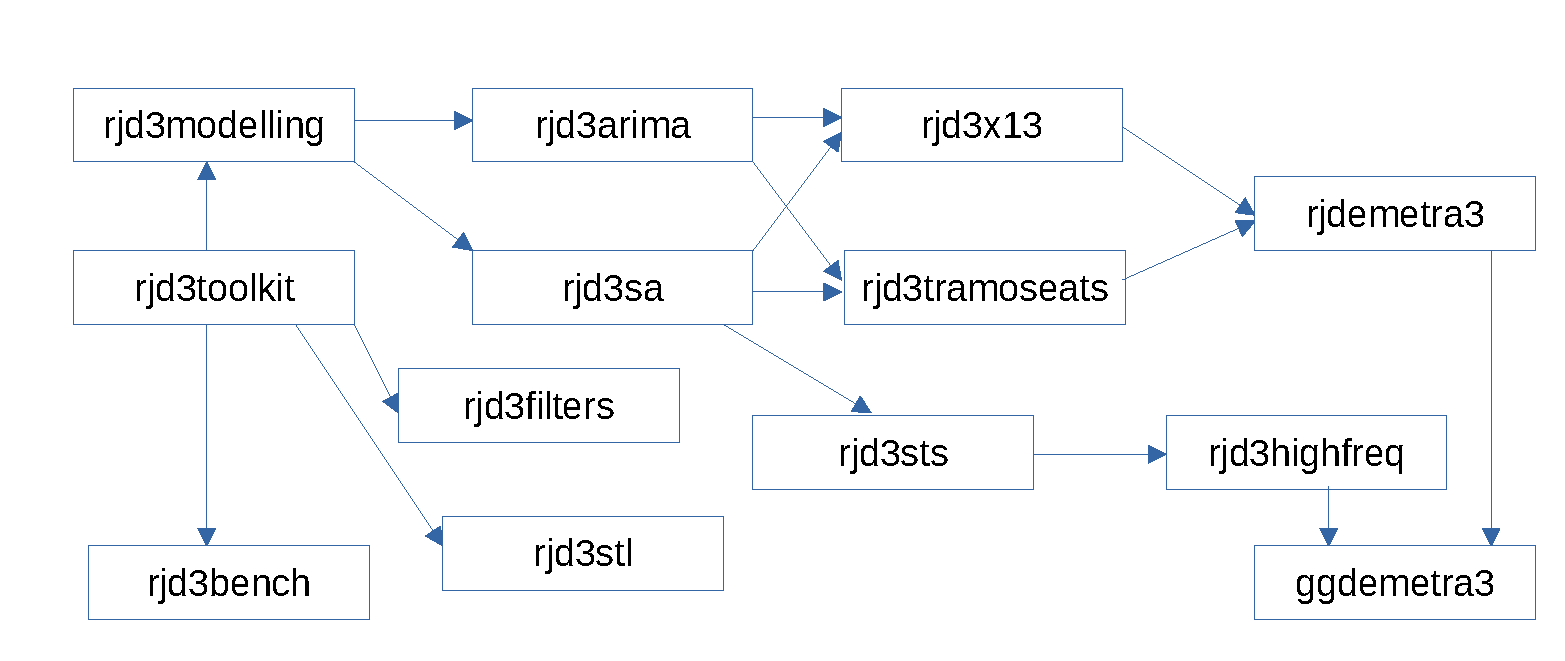
\includegraphics{img/diag.pdf}

And it's just the begining! (might change in the future)
\end{frame}

\hypertarget{utility-packages}{%
\section{Utility packages}\label{utility-packages}}

\hypertarget{rjd3toolkit}{%
\subsection{rjd3toolkit}\label{rjd3toolkit}}

\begin{frame}[fragile]{rjd3toolkit}
\protect\hypertarget{rjd3toolkit-1}{}
Contains several utility functions used in other \texttt{rjd} packages
and several functions to perform tests:

\begin{itemize}
\item
  Normality tests: Bowman-Shenton (\texttt{bowmanshenton()}),
  Doornik-Hansen (\texttt{doornikhansen()}), Jarque-Bera
  (\texttt{jarquebera()}, with more parameters than
  \texttt{tseries::jarque.bera.test()})
\item
  \bclampe Runs tests (randomness of data): mean or the median
  (\texttt{testofruns()}) or up and down runs test
  (\texttt{testofupdownruns()})
\item
  autocorrelation functions (usual, inverse, partial)
\item
  \texttt{aggregate()} to aggregate a time serie to a higher frequency
\end{itemize}
\end{frame}

\hypertarget{rjd3modelling}{%
\subsection{rjd3modelling}\label{rjd3modelling}}

\begin{frame}[fragile]{rjd3modelling}
\protect\hypertarget{rjd3modelling-1}{}
\footnotesize

\begin{itemize}
\tightlist
\item
  \bclampe create user-defined calendar and trading-days regressors:
  \texttt{calendar.new()} (create a new calendar),
  \texttt{calendar.holiday()} (add a specific holiday, e.g.~christmas),
  \texttt{calendar.easter()} (easter related day) and
  \texttt{calendar.fixedday()})
\end{itemize}

\pause

\begin{itemize}
\tightlist
\item
  \bclampe create outliers regressors (AO, LS, TC, SO, Ramp,
  intervention variables), calendar related regressors (stock, leap
  year, periodic dummies and contrasts, trigonometric variables)
  -\textgreater{} to be added quadratic ramps
\end{itemize}

\pause

\begin{itemize}
\tightlist
\item
  \bclampe  Range-mean regression test (to choose log transformation,
  \texttt{rangemean.tstat()}), Canova-Hansen (\texttt{td.ch()}) and
  trading-days f-test (\texttt{td.f()})
\end{itemize}

\pause

\begin{itemize}
\tightlist
\item
  manipulation of ARIMA models (generation, sum, decomposition,
  estimation)
\end{itemize}

\pause

\begin{itemize}
\tightlist
\item
  functions to stationarise your series \texttt{do.stationary()},
  \texttt{differences()}, \texttt{differencing.fast()}
\end{itemize}

\pause

\begin{itemize}
\tightlist
\item
  specification functions for \texttt{rjd3x13} and
  \texttt{rjd3tramoseats}
\end{itemize}
\end{frame}

\begin{frame}[fragile,allowframebreaks]{Example of a specific calendar}
\protect\hypertarget{example-of-a-specific-calendar}{}
\begin{Shaded}
\begin{Highlighting}[]
\FunctionTok{library}\NormalTok{(rjd3modelling)}
\NormalTok{fr\_cal }\OtherTok{\textless{}{-}} \FunctionTok{calendar.new}\NormalTok{()}
\FunctionTok{calendar.holiday}\NormalTok{(fr\_cal, }\StringTok{"NEWYEAR"}\NormalTok{)}
\FunctionTok{calendar.holiday}\NormalTok{(fr\_cal, }\StringTok{"EASTERMONDAY"}\NormalTok{)}
\FunctionTok{calendar.holiday}\NormalTok{(fr\_cal, }\StringTok{"MAYDAY"}\NormalTok{)}
\FunctionTok{calendar.fixedday}\NormalTok{(fr\_cal, }\AttributeTok{month =} \DecValTok{5}\NormalTok{, }\AttributeTok{day =} \DecValTok{8}\NormalTok{,}
                  \AttributeTok{start =} \StringTok{"1953{-}03{-}20"}\NormalTok{)}
\CommentTok{\# calendar.holiday(fr\_cal, "WHITMONDAY") \# Equivalent to:}
\FunctionTok{calendar.easter}\NormalTok{(fr\_cal, }\AttributeTok{offset =} \DecValTok{61}\NormalTok{)}

\FunctionTok{calendar.fixedday}\NormalTok{(fr\_cal, }\AttributeTok{month =} \DecValTok{7}\NormalTok{, }\AttributeTok{day =} \DecValTok{14}\NormalTok{)}
\CommentTok{\# calendar.holiday(fr\_cal, "ASSUMPTION")}
\FunctionTok{calendar.easter}\NormalTok{(fr\_cal, }\AttributeTok{offset =} \DecValTok{61}\NormalTok{)}
\FunctionTok{calendar.holiday}\NormalTok{(fr\_cal, }\StringTok{"ALLSAINTSDAY"}\NormalTok{)}
\FunctionTok{calendar.holiday}\NormalTok{(fr\_cal, }\StringTok{"ARMISTICE"}\NormalTok{)}
\FunctionTok{calendar.holiday}\NormalTok{(fr\_cal, }\StringTok{"CHRISTMAS"}\NormalTok{)}
\end{Highlighting}
\end{Shaded}

\footnotesize

Use \texttt{holidays()} to get the days of the holidays and
\texttt{htd()} to get the trading days regressors

\begin{Shaded}
\begin{Highlighting}[]
\FunctionTok{holidays}\NormalTok{(fr\_cal, }\StringTok{"2020{-}12{-}24"}\NormalTok{, }\DecValTok{10}\NormalTok{, }\AttributeTok{single =} \ConstantTok{TRUE}\NormalTok{)}
\end{Highlighting}
\end{Shaded}

\begin{verbatim}
##            [,1]
## 2020-12-24    0
## 2020-12-25    1
## 2020-12-26    0
## 2020-12-27    0
## 2020-12-28    0
## 2020-12-29    0
## 2020-12-30    0
## 2020-12-31    0
## 2021-01-01    1
## 2021-01-02    0
\end{verbatim}

\begin{Shaded}
\begin{Highlighting}[]
\NormalTok{s }\OtherTok{\textless{}{-}} \FunctionTok{ts}\NormalTok{(}\DecValTok{0}\NormalTok{, }\AttributeTok{start =} \DecValTok{2020}\NormalTok{, }\AttributeTok{end =} \FunctionTok{c}\NormalTok{(}\DecValTok{2020}\NormalTok{, }\DecValTok{11}\NormalTok{), }\AttributeTok{frequency =} \DecValTok{12}\NormalTok{)}
\CommentTok{\# Trading{-}days regressors (each day has a different effect, sunday as contrasts)}
\NormalTok{td\_reg }\OtherTok{\textless{}{-}} \FunctionTok{htd}\NormalTok{(fr\_cal, }\AttributeTok{s =}\NormalTok{ s, }\AttributeTok{groups =} \FunctionTok{c}\NormalTok{(}\DecValTok{1}\NormalTok{, }\DecValTok{2}\NormalTok{, }\DecValTok{3}\NormalTok{, }\DecValTok{4}\NormalTok{, }\DecValTok{5}\NormalTok{, }\DecValTok{6}\NormalTok{, }\DecValTok{0}\NormalTok{))}
\CommentTok{\# Working{-}days regressors (Monday = ... = Friday; Saturday = Sunday = contrasts)}
\NormalTok{wd\_reg }\OtherTok{\textless{}{-}} \FunctionTok{htd}\NormalTok{(fr\_cal, }\AttributeTok{s =}\NormalTok{ s, }\AttributeTok{groups =} \FunctionTok{c}\NormalTok{(}\DecValTok{1}\NormalTok{, }\DecValTok{1}\NormalTok{, }\DecValTok{1}\NormalTok{, }\DecValTok{1}\NormalTok{, }\DecValTok{1}\NormalTok{, }\DecValTok{0}\NormalTok{, }\DecValTok{0}\NormalTok{))}
\CommentTok{\# Monday = ... = Friday; Saturday; Sunday = contrasts}
\NormalTok{wd\_reg }\OtherTok{\textless{}{-}} \FunctionTok{htd}\NormalTok{(fr\_cal, }\AttributeTok{s =}\NormalTok{ s, }\AttributeTok{groups =} \FunctionTok{c}\NormalTok{(}\DecValTok{1}\NormalTok{, }\DecValTok{1}\NormalTok{, }\DecValTok{1}\NormalTok{, }\DecValTok{1}\NormalTok{, }\DecValTok{1}\NormalTok{, }\DecValTok{2}\NormalTok{, }\DecValTok{0}\NormalTok{))}
\NormalTok{wd\_reg}
\end{Highlighting}
\end{Shaded}

\begin{verbatim}
##             group-1    group-2
## Jan 2020  2.0000000  0.0000000
## Feb 2020  0.0000000  1.0000000
## Mar 2020 -1.7809251 -0.7968209
## Apr 2020  0.7809251 -0.2031791
## May 2020 -3.1554920  0.4740847
## Jun 2020  5.1554920  0.5259153
## Jul 2020  2.0000000  0.0000000
## Aug 2020 -4.0000000  0.0000000
## Sep 2020  2.0000000  0.0000000
## Oct 2020  2.0000000  1.0000000
## Nov 2020  0.0000000  0.0000000
\end{verbatim}
\end{frame}

\begin{frame}[fragile,allowframebreaks]{Example of outliers}
\protect\hypertarget{example-of-outliers}{}
\footnotesize

\begin{Shaded}
\begin{Highlighting}[]
\NormalTok{s }\OtherTok{\textless{}{-}} \FunctionTok{ts}\NormalTok{(}\DecValTok{0}\NormalTok{, }\AttributeTok{start =} \DecValTok{2000}\NormalTok{, }\AttributeTok{end =} \DecValTok{2005}\NormalTok{, }\AttributeTok{frequency =} \DecValTok{12}\NormalTok{)}
\NormalTok{ao }\OtherTok{\textless{}{-}} \FunctionTok{ao.variable}\NormalTok{(}\AttributeTok{s =}\NormalTok{ s, }\AttributeTok{date =} \StringTok{"2001{-}03{-}01"}\NormalTok{)}
\NormalTok{ls }\OtherTok{\textless{}{-}} \FunctionTok{ls.variable}\NormalTok{(}\AttributeTok{s =}\NormalTok{ s, }\AttributeTok{date =} \StringTok{"2001{-}01{-}01"}\NormalTok{)}
\NormalTok{tc }\OtherTok{\textless{}{-}} \FunctionTok{tc.variable}\NormalTok{(}\AttributeTok{s =}\NormalTok{ s, }\AttributeTok{date =} \StringTok{"2001{-}01{-}01"}\NormalTok{, }\AttributeTok{rate =} \FloatTok{0.7}\NormalTok{)}
\NormalTok{so }\OtherTok{\textless{}{-}} \FunctionTok{so.variable}\NormalTok{(}\AttributeTok{s =}\NormalTok{ s, }\AttributeTok{date =} \StringTok{"2003{-}05{-}01"}\NormalTok{)}
\NormalTok{ramp }\OtherTok{\textless{}{-}} \FunctionTok{ramp.variable}\NormalTok{(}\AttributeTok{s =}\NormalTok{ s, }\AttributeTok{range =} \FunctionTok{c}\NormalTok{(}\StringTok{"2001{-}01{-}01"}\NormalTok{, }\StringTok{"2001{-}12{-}01"}\NormalTok{))}
\FunctionTok{plot}\NormalTok{(}\FunctionTok{ts.union}\NormalTok{(ao, ls, tc, so, ramp), }\AttributeTok{plot.type =} \StringTok{"single"}\NormalTok{,}
     \AttributeTok{col =} \FunctionTok{c}\NormalTok{(}\StringTok{"red"}\NormalTok{,}\StringTok{"lightgreen"}\NormalTok{,}\StringTok{"orange"}\NormalTok{,}\StringTok{"blue"}\NormalTok{,}\StringTok{"black"}\NormalTok{))}
\end{Highlighting}
\end{Shaded}

\begin{center}\includegraphics{img/slides-outplot-1} \end{center}
\end{frame}

\begin{frame}{Benchmark of ARIMA estimations}
\protect\hypertarget{benchmark-of-arima-estimations}{}
More than 20 time faster in median!

\footnotesize

\begin{center}\includegraphics[height=0.9\textheight]{img/slides-performance-arima-1} \end{center}
\end{frame}

\hypertarget{rjd3sa}{%
\subsection{rjd3sa}\label{rjd3sa}}

\begin{frame}[fragile]{rjd3sa (1)}
\protect\hypertarget{rjd3sa-1}{}
Seasonality tests:

\begin{itemize}
\item
  Canova-Hansen (\texttt{seasonality.canovahansen()})
\item
  \bclampe X-12 combined test (\texttt{seasonality.combined()})
\item
  F-test on seasonal dummies (\texttt{seasonality.f()})
\item
  Friedman Seasonality Test (\texttt{seasonality.friedman()})
\item
  Kruskall-Wallis Seasonality Test
  (\texttt{seasonality.kruskalwallis()})
\item
  \bclampe Periodogram Seasonality Test
  (\texttt{seasonality.periodogram()})
\item
  QS Seasonality Test (\texttt{seasonality.qs()})
\end{itemize}
\end{frame}

\begin{frame}[fragile]{rjd3sa (2)}
\protect\hypertarget{rjd3sa-2}{}
\bcattention Always correct the trend and remove the mean before
seasonality tests: \footnotesize

\begin{Shaded}
\begin{Highlighting}[]
\FunctionTok{library}\NormalTok{(rjd3sa)}
\NormalTok{y }\OtherTok{\textless{}{-}} \FunctionTok{diff}\NormalTok{(rjd3toolkit}\SpecialCharTok{::}\NormalTok{ABS}\SpecialCharTok{$}\NormalTok{X0.}\DecValTok{2}\NormalTok{.}\DecValTok{09}\NormalTok{.}\FloatTok{10.}\NormalTok{M, }\DecValTok{1}\NormalTok{); y }\OtherTok{\textless{}{-}}\NormalTok{ y }\SpecialCharTok{{-}} \FunctionTok{mean}\NormalTok{(y)}
\CommentTok{\# Or:}
\NormalTok{y }\OtherTok{\textless{}{-}}\NormalTok{ rjd3modelling}\SpecialCharTok{::}\FunctionTok{differences}\NormalTok{(rjd3toolkit}\SpecialCharTok{::}\NormalTok{ABS}\SpecialCharTok{$}\NormalTok{X0.}\DecValTok{2}\NormalTok{.}\DecValTok{09}\NormalTok{.}\FloatTok{10.}\NormalTok{M)}
\FunctionTok{seasonality.f}\NormalTok{(y)}
\end{Highlighting}
\end{Shaded}

\begin{verbatim}
## Value:  378.9234 
## P-Value:  0.0000
\end{verbatim}

\begin{Shaded}
\begin{Highlighting}[]
\FunctionTok{seasonality.friedman}\NormalTok{(y)}
\end{Highlighting}
\end{Shaded}

\begin{verbatim}
## Value:  298.2529 
## P-Value:  0.0000
\end{verbatim}

\begin{Shaded}
\begin{Highlighting}[]
\FunctionTok{seasonality.kruskalwallis}\NormalTok{(y)}
\end{Highlighting}
\end{Shaded}

\begin{verbatim}
## Value:  319.9801 
## P-Value:  0.0000
\end{verbatim}

\begin{Shaded}
\begin{Highlighting}[]
\FunctionTok{seasonality.combined}\NormalTok{(y)}
\end{Highlighting}
\end{Shaded}

\begin{verbatim}
## $seasonality
## [1] "PRESENT"
## 
## $kruskalwallis
## $kruskalwallis$value
## [1] 319.9801
## 
## $kruskalwallis$pvalue
## [1] 0
## 
## $kruskalwallis$description
## [1] "Chi2 with 11.0 degrees of freedom "
## 
## 
## $stable
## $stable$SSM
## [1] 69596527
## 
## $stable$dfM
## [1] 11
## 
## $stable$SSR
## [1] 6721009
## 
## $stable$dfR
## [1] 412
## 
## $stable$test
## Value:  387.8445 
## P-Value:  0.0000 
## 
## 
## $evolutive
## $evolutive$SSM
## [1] 2145849
## 
## $evolutive$dfM
## [1] 34
## 
## $evolutive$SSR
## [1] 3800578
## 
## $evolutive$dfR
## [1] 374
## 
## $evolutive$test
## Value:  6.210723 
## P-Value:  0.0000
\end{verbatim}
\end{frame}

\hypertarget{seasonal-adjustment-packages}{%
\section{Seasonal adjustment
packages}\label{seasonal-adjustment-packages}}

\hypertarget{rjd3arima}{%
\subsection{rjd3arima}\label{rjd3arima}}

\begin{frame}[fragile]{rjd3arima}
\protect\hypertarget{rjd3arima-1}{}
\texttt{rjd3arima} is devoted to formatting the output of Arima related
results
\end{frame}

\hypertarget{rjd3x13-and-rjd3tramoseats}{%
\subsection{rjd3x13 and
rjd3tramoseats}\label{rjd3x13-and-rjd3tramoseats}}

\begin{frame}[fragile]{Common functions}
\protect\hypertarget{common-functions}{}
Common functions (defined in \texttt{rjd3modelling}) to set the
specification of the preprocessing:

\texttt{set\_arima()}, \texttt{set\_automodel()}, \texttt{set\_basic()},
\texttt{set\_easter()}, \texttt{set\_estimate()},
\texttt{set\_outlier()}, \texttt{set\_tradingdays()},
\texttt{set\_transform()}, \texttt{add\_outlier()} and
\texttt{remove\_outlier()}, \texttt{add\_ramp()},
\texttt{remove\_ramp()}, \texttt{add\_usrdefvar()}
\end{frame}

\begin{frame}[fragile]{rjd3x13}
\protect\hypertarget{rjd3x13}{}
Main functions:

\begin{itemize}
\item
  Specification: created with \texttt{spec\_x11\_default()},
  \texttt{spec\_x13\_default()}, \texttt{spec\_regarima\_default()} and
  customized with \texttt{rjd3modelling} functions + \texttt{set\_x11()}
\item
  Apply SA model with \texttt{x11()}, \texttt{x13()},
  \texttt{fast.x13()}
\item
  ARIMA modelling with \texttt{regarima()}, \texttt{fast.regarima()}
\item
  \bclampe Refresh policies: \texttt{regarima.refresh()} and
  \texttt{x13.refresh()}
\end{itemize}
\end{frame}

\begin{frame}[fragile]{Performance}
\protect\hypertarget{performance}{}
In median: \texttt{RJDemetra} more 3 time faster than \texttt{seasonal}
and \texttt{rjdemetra3} more than 12 time faster than \texttt{seasonal}!

\begin{center}\includegraphics[height=0.9\textheight]{img/slides-performance-1} \end{center}
\end{frame}

\begin{frame}[fragile,allowframebreaks]{Exemple}
\protect\hypertarget{exemple}{}
\scriptsize

\begin{Shaded}
\begin{Highlighting}[]
\FunctionTok{library}\NormalTok{(rjd3modelling);}\FunctionTok{library}\NormalTok{(rjd3x13)}
\NormalTok{y }\OtherTok{\textless{}{-}}\NormalTok{ rjd3toolkit}\SpecialCharTok{::}\NormalTok{ABS}\SpecialCharTok{$}\NormalTok{X0.}\DecValTok{2}\NormalTok{.}\DecValTok{09}\NormalTok{.}\FloatTok{10.}\NormalTok{M}
\NormalTok{spec }\OtherTok{\textless{}{-}} \FunctionTok{spec\_x13\_default}\NormalTok{(}\StringTok{"rsa5c"}\NormalTok{) }\SpecialCharTok{|\textgreater{}} \FunctionTok{set\_easter}\NormalTok{(}\AttributeTok{type =} \StringTok{"unused"}\NormalTok{) }\SpecialCharTok{|\textgreater{}} 
  \FunctionTok{set\_outlier}\NormalTok{(}\AttributeTok{outliers.type =} \FunctionTok{c}\NormalTok{(}\StringTok{"AO"}\NormalTok{, }\StringTok{"LS"}\NormalTok{)) }\SpecialCharTok{|\textgreater{}} 
  \FunctionTok{set\_tradingdays}\NormalTok{(}\AttributeTok{test =} \StringTok{"None"}\NormalTok{) }\SpecialCharTok{|\textgreater{}} \FunctionTok{set\_x11}\NormalTok{(}\AttributeTok{henderson.filter =} \DecValTok{13}\NormalTok{) }\SpecialCharTok{|\textgreater{}} 
  \FunctionTok{add\_outlier}\NormalTok{(}\AttributeTok{type =} \StringTok{"TC"}\NormalTok{, }\AttributeTok{date =} \StringTok{"2000{-}06{-}01"}\NormalTok{,}
              \AttributeTok{name =} \StringTok{"My TC in 2000{-}06"}\NormalTok{) }
\NormalTok{m }\OtherTok{=}\NormalTok{ rjd3x13}\SpecialCharTok{::}\FunctionTok{x13}\NormalTok{(y, spec)}
\NormalTok{m}\SpecialCharTok{$}\NormalTok{result}\SpecialCharTok{$}\NormalTok{preprocessing}
\end{Highlighting}
\end{Shaded}

\begin{verbatim}
## Log-transformation: yes 
## SARIMA model:  (0,1,2) (1,1,1) 
## 
## Coefficients
##           Estimate Std. Error  T-stat
## theta(1)  -1.01804    0.07639 -13.326
## theta(2)   0.20863    0.05378   3.879
## bphi(1)   -0.26680    0.05399  -4.942
## btheta(1) -0.77559    0.05384 -14.405
## 
## Regression model:
##                   Estimate Std. Error T-stat
## monday           -0.011247   0.004004 -2.809
## tuesday           0.005870   0.004013  1.463
## wednesday        -0.002002   0.004003 -0.500
## thursday          0.014483   0.004021  3.602
## friday            0.001577   0.004023  0.392
## saturday          0.011465   0.003996  2.869
## lp                0.037501   0.010994  3.411
## easter            0.053486   0.008319  6.429
## My TC in 2000-06  0.022947   0.023666  0.970
## Number of observations:  425 
## Number of effective observations:  412 
## Number of parameters:  14 
## 
## Loglikelihood:  763.5143 
## Adjusted loglikelihood:  -2104.113 
## 
## Standard error of the regression (ML estimate):  0.03757223 
## AIC:  4236.225 
## AICC:  4237.283 
## BIC:  4292.519
\end{verbatim}

\begin{Shaded}
\begin{Highlighting}[]
\CommentTok{\# Also summary function}
\CommentTok{\# summary(m)}
\FunctionTok{plot}\NormalTok{(m)}
\end{Highlighting}
\end{Shaded}

\begin{center}\includegraphics{img/slides-x13-1} \end{center}
\end{frame}

\hypertarget{rjd3tramoseats}{%
\subsection{rjd3tramoseats}\label{rjd3tramoseats}}

\begin{frame}[fragile]{rjd3tramoseats}
\protect\hypertarget{rjd3tramoseats-1}{}
Main functions:

\begin{itemize}
\item
  Specification: created with \texttt{spec\_tramoseats\_default()},
  \texttt{spec\_tramo\_default()} and customized with \texttt{rjd3arima}
  functions + \texttt{set\_seats()}
\item
  Apply model with \texttt{tramoseats()}, \texttt{fast.tramoseats()},
  \texttt{tramo()}, \texttt{fast.tramo()}
\item
  \bclampe Refresh policies: \texttt{tramo.refresh()} and
  \texttt{tramoseats.refresh()}
\end{itemize}

Example:

\begin{Shaded}
\begin{Highlighting}[]
\NormalTok{spec }\OtherTok{\textless{}{-}} \FunctionTok{spec\_tramoseats\_default}\NormalTok{(}\StringTok{"rsafull"}\NormalTok{) }\SpecialCharTok{|\textgreater{}} 
  \FunctionTok{set\_easter}\NormalTok{(}\AttributeTok{type =} \StringTok{"IncludeEasterMonday"}\NormalTok{) }\SpecialCharTok{|\textgreater{}} 
  \FunctionTok{set\_tradingdays}\NormalTok{(}\AttributeTok{test =} \StringTok{"Separate\_T"}\NormalTok{) }\SpecialCharTok{|\textgreater{}} 
  \FunctionTok{set\_seats}\NormalTok{(}\AttributeTok{algorithm =} \StringTok{"KalmanSmoother"}\NormalTok{)}
\NormalTok{m }\OtherTok{\textless{}{-}}\NormalTok{ rjd3tramoseats}\SpecialCharTok{::}\FunctionTok{tramoseats}\NormalTok{(y, spec)}
\end{Highlighting}
\end{Shaded}
\end{frame}

\hypertarget{rjdemetra3}{%
\subsection{rjdemetra3}\label{rjdemetra3}}

\begin{frame}[fragile]{rjdemetra3}
\protect\hypertarget{rjdemetra3-1}{}
Functions to manipulate JDemetra+ workspaces:

\begin{itemize}
\item
  Still in construction: you can load an existing workspace but not
  create a new one (use \texttt{jws.load()} for example)
\item
  Will contain all the functionalities of \texttt{rjdworkspace} (more
  manipulation of workspaces)
\end{itemize}
\end{frame}

\hypertarget{rjd3highfreq-and-rjd3stl}{%
\subsection{rjd3highfreq and rjd3stl}\label{rjd3highfreq-and-rjd3stl}}

\begin{frame}[fragile]{rjd3highfreq and rjd3stl}
\protect\hypertarget{rjd3highfreq-and-rjd3stl-1}{}
Seasonal adjustment of high frequency data:

\begin{itemize}
\item
  \bclampe fractional and multi airline decomposition
\item
  \bclampe Extension of X-11 decomposition with non integer periodicity
\end{itemize}

\texttt{rjd3stl}: STL, MSTL, ISTL, loess

See next presentation of Anna Smyk
\end{frame}

\hypertarget{other-packages}{%
\section{Other packages}\label{other-packages}}

\hypertarget{ggdemetra3}{%
\subsection{ggdemetra3}\label{ggdemetra3}}

\begin{frame}[fragile,allowframebreaks]{ggdemetra3}
\protect\hypertarget{ggdemetra3-1}{}
Like \texttt{ggdemetra} but compatible with \texttt{rjdemetra3}: ggplot2
to add seasonal adjustment statistics to your plot,\texttt{autoplot()}
functions\ldots{} Also compatible with high-frequency methods (WIP):
\footnotesize

\begin{Shaded}
\begin{Highlighting}[]
\FunctionTok{library}\NormalTok{(ggdemetra3)}
\NormalTok{spec }\OtherTok{\textless{}{-}} \FunctionTok{spec\_x13\_default}\NormalTok{(}\StringTok{"rsa3"}\NormalTok{) }\SpecialCharTok{|\textgreater{}} 
  \FunctionTok{set\_tradingdays}\NormalTok{(}\AttributeTok{option =} \StringTok{"WorkingDays"}\NormalTok{)}
\FunctionTok{ggplot}\NormalTok{(}\AttributeTok{data =}\NormalTok{ ipi\_c\_eu\_df, }\AttributeTok{mapping =} \FunctionTok{aes}\NormalTok{(}\AttributeTok{x =}\NormalTok{ date, }\AttributeTok{y =}\NormalTok{ FR)) }\SpecialCharTok{+}
    \FunctionTok{geom\_line}\NormalTok{() }\SpecialCharTok{+}
    \FunctionTok{labs}\NormalTok{(}\AttributeTok{title =} \StringTok{"SA {-} IPI{-}FR"}\NormalTok{,}
         \AttributeTok{x =} \ConstantTok{NULL}\NormalTok{, }\AttributeTok{y =} \ConstantTok{NULL}\NormalTok{) }\SpecialCharTok{+}
  \FunctionTok{geom\_sa}\NormalTok{(}\AttributeTok{component =} \StringTok{"y\_f(12)"}\NormalTok{, }\AttributeTok{linetype =} \DecValTok{2}\NormalTok{,}
          \AttributeTok{spec =}\NormalTok{ spec) }\SpecialCharTok{+} 
  \FunctionTok{geom\_sa}\NormalTok{(}\AttributeTok{component =} \StringTok{"sa"}\NormalTok{, }\AttributeTok{color =} \StringTok{"red"}\NormalTok{) }\SpecialCharTok{+}
  \FunctionTok{geom\_sa}\NormalTok{(}\AttributeTok{component =} \StringTok{"sa\_f"}\NormalTok{, }\AttributeTok{color =} \StringTok{"red"}\NormalTok{, }\AttributeTok{linetype =} \DecValTok{2}\NormalTok{) }\SpecialCharTok{+}
  \FunctionTok{geom\_outlier}\NormalTok{(}\AttributeTok{geom =} \StringTok{"label\_repel"}\NormalTok{,}
               \AttributeTok{coefficients =} \ConstantTok{TRUE}\NormalTok{,}
               \AttributeTok{ylim =} \FunctionTok{c}\NormalTok{(}\ConstantTok{NA}\NormalTok{, }\DecValTok{65}\NormalTok{), }\AttributeTok{force =} \DecValTok{10}\NormalTok{,}
               \AttributeTok{arrow =} \FunctionTok{arrow}\NormalTok{(}\AttributeTok{length =} \FunctionTok{unit}\NormalTok{(}\FloatTok{0.03}\NormalTok{, }\StringTok{"npc"}\NormalTok{),}
                             \AttributeTok{type =} \StringTok{"closed"}\NormalTok{, }\AttributeTok{ends =} \StringTok{"last"}\NormalTok{),}
               \AttributeTok{digits =} \DecValTok{2}\NormalTok{)}
\end{Highlighting}
\end{Shaded}

\begin{center}\includegraphics{img/slides-ggdemetra3-1} \end{center}
\end{frame}

\begin{frame}[fragile]{Plot from an existing model}
\protect\hypertarget{plot-from-an-existing-model}{}
\footnotesize

\begin{Shaded}
\begin{Highlighting}[]
\NormalTok{mod }\OtherTok{\textless{}{-}}\NormalTok{ rjd3x13}\SpecialCharTok{::}\FunctionTok{x13}\NormalTok{(y, spec)}
\CommentTok{\# siratioplot(mod) \# SI Ratio plot}
\FunctionTok{autoplot}\NormalTok{(mod) }\CommentTok{\# autoplot}
\end{Highlighting}
\end{Shaded}

\begin{center}\includegraphics{img/slides-ggdemetra3-mod-1} \end{center}
\end{frame}

\hypertarget{rjd3filters}{%
\subsection{rjd3filters}\label{rjd3filters}}

\begin{frame}[fragile]{\texttt{rjd3filters}}
\protect\hypertarget{rjd3filters-1}{}
\begin{itemize}
\tightlist
\item
  \bclampe easily create/combine/apply moving averages
  \texttt{moving\_average()} (much more general than
  \texttt{stats::filter()}) and study their properties: plot
  coefficients (\texttt{plot\_coef()}), gain (\texttt{plot\_gain()}),
  phase-shift (\texttt{plot\_phase()}) and different statics
  (\texttt{diagnostic\_matrix()})
\end{itemize}

Goal: manipulate moving averages \[
M_\theta(X_t)=\sum_{k=-p}^{+f}\theta_kX_{t+k} = 
\left(\sum_{k=-p}^{+f}\theta_k B^{-k}\right)X_{t}\text{ with }B^k=X_{t-k}
\] (Currently in \faIcon{r-project} you can only limited forms of MA)

\pause

\begin{itemize}
\tightlist
\item
  \bclampe Lots of complicated and interesting things around trend-cycle
  estimates
\end{itemize}

See my presentation at \textbf{SAPW 2022} Concurrent Session 5b - Trends
\url{https://community.amstat.org/governmentstatisticssection/conferences/pastconference210/seasonal-adjustment-practitioners-workshop-2022}
\end{frame}

\hypertarget{rjd3sts-and-rjd3bench}{%
\subsection{rjd3sts and rjd3bench}\label{rjd3sts-and-rjd3bench}}

\begin{frame}[fragile]{rjd3sts and rjd3bench}
\protect\hypertarget{rjd3sts-and-rjd3bench-1}{}
\texttt{rjd3sts} Interface to structural time series and state space
models

Several examples available here
\url{https://github.com/palatej/test_rjd3sts}

\texttt{rjd3bench} Benchmarking and temporal disaggregation

Several examples here: \url{https://github.com/palatej/test_rjd3bench}
\end{frame}

\hypertarget{conclusion}{%
\section{Conclusion}\label{conclusion}}

\begin{frame}{Conclusion}
\protect\hypertarget{conclusion-1}{}
With JDemetra+ 3.0, lots of new \faIcon{r-project} packages are coming:

\begin{itemize}
\item
  On time series analysis and seasonal adjustment (much faster than
  standard packages)
\item
  New developments on seasonal adjustment will be available
  (e.g.~high-frequency data)
\item
  Allow to create new trainings thanks to a deeper acces to all the
  functionalities of JDemetra+
\end{itemize}

Many ways to contribute:

\begin{itemize}
\item
  Testing it and reporting issues
\item
  Developping new tools (other packages, new functions, etc.)
\end{itemize}
\end{frame}

\begin{frame}[noframenumbering]{Thank you for your attention}
\protect\hypertarget{thank-you-for-your-attention}{}
Packages \faIcon{r-project}{}:

\begin{columns}[T]
\begin{column}{0.4\textwidth}
\href{https://github.com/palatej/rjd3toolkit}{\faGithub{} palatej/rjd3toolkit}

\href{https://github.com/palatej/rjd3modelling}{\faGithub{} palatej/rjd3modelling}

\href{https://github.com/palatej/rjd3sa}{\faGithub{} palatej/rjd3sa}

\href{https://github.com/palatej/rjd3arima}{\faGithub{} palatej/rjd3arima}

\href{https://github.com/palatej/rjd3x13}{\faGithub{} palatej/rjd3x13}

\href{https://github.com/palatej/rjd3tramoseats}{\faGithub{} palatej/rjd3tramoseats}

\href{https://github.com/palatej/rjdemetra3}{\faGithub{} palatej/rjdemetra3}
\end{column}

\begin{column}{0.5\textwidth}
\href{https://github.com/palatej/rjdfilters}{\faGithub{} palatej/rjdfilters}

\href{https://github.com/palatej/rjd3sts}{\faGithub{} palatej/rjd3sts}

\href{https://github.com/palatej/rjd3stl}{\faGithub{} palatej/rjd3stl}

\href{https://github.com/palatej/rjd3highfreq}{\faGithub{} palatej/rjd3highfreq}

\href{https://github.com/palatej/rjd3bench}{\faGithub{} palatej/rjd3bench}

\href{https://github.com/AQLT/ggdemetra3}{\faGithub{} AQLT/ggdemetra3}
\end{column}
\end{columns}
\end{frame}

\end{document}
